\subsection{Enumerating all possible inputs for a specific regular expression}

\renewcommand{\CURPATH}{regexp/SMT}

Regular expression if first converted to \ac{FSM} before matching.
Hence, many \ac{RE} libraries has two functions: ``compile'' and ``execute''
(when you match many strings against single \ac{RE}, no need to recompile it to \ac{FSM} each time).

And I've found this website, which can visualize \ac{FSM} for a regular expression.
\url{http://hokein.github.io/Automata.js/}.
This is fun!

This \ac{FSM} (\ac{DFA}) is for the expression \TT{(dark|light)?(red|blue|green)(ish)?}

\begin{figure}[H]
\centering
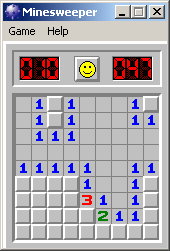
\includegraphics[scale=0.6]{\CURPATH/1.png}
\caption{}
\end{figure}

% FSM.png
Another version: URL.

Accepting states are in double circles, these are the states where matching process stops.

How can we generate an input string which regular expression would match?
In other words, which inputs \ac{FSM} would accept?
This task is surprisingly simple for SMT-solver.

We just define a transition function.
For each pair (state, input) it defines new state.

\ac{FSM} has been visualized by the website mentioned above, and I used this information to write ``transition()'' function.

Then we chain transition functions... then we try a chain for all lengths in range of 2..14.

\lstinputlisting{\CURPATH/re_MK85.py}

Results:

\lstinputlisting{\CURPATH/res.txt}

As simple as this.

The source code for Z3Py: \url{...re_Z3.py}.

% TODO \gls
It can be said, what we did is enumeration of all paths between two vertices of a digraph (representing \ac{FSM}).

Also, the ``transition()'' function itself can act as a RE matcher, with no relevance to SMT solver(s).
Just feed input characters to it and track state.
Whenever you hit one of accepting states, return ``match'', whenever you hit \TT{INVALID\_STATE}, return ``no match''.

